\documentclass[a4paper,11pt]{article}
\usepackage{geometry}
\usepackage{setspace}
\usepackage{graphicx}
\usepackage[utf8]{inputenc}
\usepackage{helvet}
\usepackage{amsmath}
\usepackage[style=apa, backend=biber]{biblatex}
\addbibresource{references.bib}
\usepackage{subcaption} 
\usepackage{float}
\usepackage{amsmath} % For math symbols
\usepackage{amsfonts} % For better math fonts
\usepackage{setspace}
\onehalfspacing
\usepackage{subcaption}
\usepackage{fancyhdr} % For custom headers and footers

 
\geometry{left=2.5cm, right=2.5cm, top=3cm, bottom=3cm}
% Setting the page margins
\pagestyle{fancy}
\fancyhf{} % Clear all header and footer fields
\fancyhead[L]{ADLS} % Left-aligned text
\fancyhead[C]{FS25} % Center-aligned text
\fancyhead[R]{Krymowski, Schibli} % Right-aligned text
\fancyfoot[R]{\thepage} % Right footer with page number
% Using Helvetica font for a modern look
\renewcommand{\familydefault}{\sfdefault}  
\begin{document}
 
% Titlepage
\begin{titlepage}
    \begin{center}
        \singlespacing
 
        \vspace*{2cm}
 
        \textbf{\large ZURICH UNIVERSITY OF APPLIED SCIENCES} \\
        \textbf{\large DEPARTMENT LIFE SCIENCES AND FACILITY MANAGEMENT} \\
        \textbf{\large INSTITUTE FOR COMPUTATIONAL LIFE SCIENCE} \\
 
        \vspace{4cm}
        \textbf{\Large Assignment 1 - DSHEALTH} \\
        \vspace{2cm}
        \textbf{\Large Detection of Pneumonia with the Kaggle Dataset: Pediatric Pneumonia Chest X-ray} \\
        \vspace{0.5cm}
        
 
        \vspace{5cm}
 
        \textbf{\large by} \\
        \textbf{\large Meggie Krymowski, Alexandra Schibli} \\
        \textbf{\large BSc Applied Digital Life Sciences 2022} \\
 
        \end{center}
        \vfill
        \begin{flushleft}
        \textbf{\large Corrector:} \\
        \textbf{\large Norman Juchler} \\
        \end{flushleft}
\end{titlepage}
\setlength{\parindent}{0pt}
 
% Abstract
%\newpage
%\begin{abstract}
   
%\end{abstract}
 \thispagestyle{empty}
 
% Table of contents
\newpage
\thispagestyle{empty}
\tableofcontents
\newpage

%Intoduction
\setcounter{page}{1}


\section{Introduction}
Pneumonia, a severe respiratory infection caused by bacteria, viruses, or fungi, inflames lung air sacs, affecting approximately 450 million people annually and causing 4 million deaths, with 740,180 children under 5 dying in 2019, per the World Health Organization (WHO) (\cite{who_pneumonia_2022}). Symptoms like fever, cough with phlegm, extreme fatigue, and breathing difficulty often start mildly but can worsen rapidly, especially in vulnerable groups such as the elderly, infants, and those with weakened immune systems, though anyone can be affected. In Switzerland, pneumonia affects 42,000 people yearly, with a hospital mortality rate of 7.3\%  xxxxxxx(Source: Swiss Federal Office of Public Health)
. The infection obstructs lung structures with pus or fluid, impairing oxygen intake, and is typically treated with antibiotics and symptomatic relief, though recovery may take days. Traditional diagnosis via chest X-rays and radiologist review is time-consuming and error-prone, particularly in resource-limited settings with scarce skilled professionals. Recent advancements in medical imaging and artificial intelligence (AI), particularly Convolutional Neural Networks (CNNs), have enabled automated pneumonia detection with high accuracy, often outperforming radiologists in controlled settings (\cite{kermany_identifying_2018}). However, real-world applicability across diverse populations and imaging conditions remains underexplored, and standardized image preprocessing techniques to enhance model performance are lacking. Early detection is critical to prevent complications like sepsis or acute respiratory distress syndrome (ARDS). This project aims to find the best-fitting CNN model for classifying pneumonia and normal chest X-rays from a given dataset, using data augmentation for diversity and cross-validation for reliability, optimizing accuracy, sensitivity, and specificity.

\section{Materials}
The main dataset used in this project was the Pediatric Chest X-ray dataset by Kermany et al., available on Kaggle~\cite{kaggle_1_2020}. It contains a total of 5,856 chest X-ray images of pediatric patients, each labeled as either ``normal'' or ``pneumonia.'' The dataset is unbalanced: around 1,583 images show normal lungs, while about 4,273 images show pneumonia. This imbalance reflects real-world conditions, where X-rays are more often taken when pneumonia is suspected.

\vspace{0.2cm}To evaluate the generalization of our models, we used a second, external dataset for validation. This dataset also comes from Kaggle and includes 180 X-ray images (90 normal and 90 with pneumonia). It was used only for final testing after training.

\section{Methodology}

\subsection{Data Exploration}
We started our project by exploring the structure and content of the Pediatric Chest X-ray dataset. The dataset includes clear and well-labeled images. A clear class imbalance was identified: approximately 1,500 images were labeled as Normal, while over 4,300
were labeled as Pneumonia, resulting in a 1:2.9 ratio. Such an imbalance is typical in clinical datasets, as X-rays are predominantly taken when disease is suspected. A visual check of the images showed noticeable differences between healthy and infected lungs, especially in terms of texture and brightness. This gave us confidence that deep learning could be used to learn from these features.

\subsection{Preprocessing and Augmentation}
To prepare the images for training and testing, we used two transformation pipelines. These were created with PyTorch’s \texttt{transforms.Compose} function. For training, we added several data augmentation steps to help the model generalize better. For testing and validation, we only applied basic preprocessing to keep the data consistent.

The training transformations included:
\begin{itemize}
    \begin{itemize}
        \item \texttt{Grayscale(num\_output\_channels=1)}: Converts the image to single-channel grayscale, reducing input dimensionality from three channels (RGB) to one, as X-rays are inherently grayscale.
        \item \texttt{Resize((128, 128))}: Resizes the image to 128$\times$128 pixels to standardize input size, reduce memory usage, and speed up training.
        \item \texttt{RandomHorizontalFlip(p=0.5)}: Flips the image horizontally with a 50\% probability, mimicking the natural left/right symmetry in X-rays.
        \item \texttt{RandomVerticalFlip(p=0.1)}: Flips the image vertically with a 10\% probability, simulating rare orientation variations.
        \item \texttt{RandomRotation(15)}: Rotates the image by a random angle between -15 and +15 degrees, accounting for slight differences in patient positioning.
        \item \texttt{RandomAffine(degrees=0, translate=(0.05, 0.05), scale=(0.95, 1.05))}: Applies small translations (5\% shift) and scaling (5\% zoom in/out), simulating minor positional variations in X-ray imaging.
        \item \texttt{ToTensor()}: Converts the image to a PyTorch tensor with shape (C, H, W), where C=1, H=128, and W=128.
        \item \texttt{Normalize(mean=[0.5], std=[0.5])}: Normalizes pixel values to the range [-1, 1], ensuring consistent input distributions for training stability.
    \end{itemize}
\end{itemize}

These transformations were applied automatically while loading the data, using the \texttt{ImageFolder} class. This method is efficient because it does not store extra images, but instead changes them each time during training. It also helps the model learn from more diverse examples, especially from the minority class (normal).

\subsection{Handling Class Imbalance}
Because there are much more pneumonia cases than normal cases in the dataset, we had to deal with this imbalance. If not handled, the model would learn to mostly predict pneumonia and ignore the minority class. To solve this, we calculated class weights based on how many samples each class had. The formula used was:

\[
\text{class\_weight}[i] = \frac{N}{C \cdot n_i}
\]

Here, \(N\) is the total number of training samples, \(C\) is the number of classes (2 in our case), and \(n_i\) is the number of samples in each class.

From these class weights, we computed a \texttt{pos\_weight} value for PyTorch’s \texttt{BCEWithLogitsLoss} function. This value helps the model give more attention to the minority class (Normal). The formula is:

\[
\text{pos\_weight} = \frac{\text{class\_weight}_{\text{Normal}}}{\text{class\_weight}_{\text{Pneumonia}}}
\]

This means that errors in detecting pneumonia (false negatives) are punished more strongly during training. This is especially important in medical use cases, where missing a pneumonia case can be dangerous for the patient.

\section{Model Building}
To test our models fairly, we used two different ways to split the data. The first split used 60\% of the data for training, 20\% for validation during training, and 20\% for testing. This is called the internal split. In the second setup, we used the same internal split but added an extra external dataset with 180 images (90 normal and 90 pneumonia) to test the generalization of our models on new data. This dataset came from a different Kaggle source and was not used during training.

\subsection{Model Architectures}
We tested two deep learning models for the task of classifying chest X-rays as normal or pneumonia: a custom-built convolutional network called FourLayerCNN and a modified ResNet18 model using transfer learning.

\subsubsection{FourLayerCNN}
The FourLayerCNN was designed especially for grayscale X-ray images of size 128×128. It contains four convolutional blocks. Each block includes a convolutional layer, followed by batch normalization, a ReLU activation, and a max-pooling operation. These blocks help the model extract important visual features while keeping the model small and fast. After the convolutional part, the output is flattened and passed through a fully connected layer with 128 units. A dropout layer is used here to reduce overfitting by randomly turning off some neurons during training. Finally, a single output neuron produces a prediction score that indicates whether the input image shows signs of pneumonia.
Table~\ref{tab:cnn_architecture} provides a detailed overview of the architecture. It lists the layers in order, the size of their outputs, and the number of trainable parameters. As shown, the model has approximately 2.49 million trainable parameters. This makes it relatively lightweight and well-suited for small to medium-sized medical datasets like ours.

\begin{table}[H]
\centering
\caption{FourLayerCNN Architecture}
\label{tab:cnn_architecture}
\begin{tabular}{|l|c|r|}
\hline
\textbf{Layer} & \textbf{Output Shape} & \textbf{Number of Parameters} \\
\hline
Input & (None, 128, 128, 1) & 0 \\
Conv2D (32 filters, 3×3) & (None, 128, 128, 32) & 320 \\
MaxPooling2D (2×2) & (None, 64, 64, 32) & 0 \\
Conv2D (64 filters, 3×3) & (None, 64, 64, 64) & 18,496 \\
MaxPooling2D (2×2) & (None, 32, 32, 64) & 0 \\
Conv2D (128 filters, 3×3) & (None, 32, 32, 128) & 73,856 \\
MaxPooling2D (2×2) & (None, 16, 16, 128) & 0 \\
Conv2D (256 filters, 3×3) & (None, 16, 16, 256) & 295,168 \\
MaxPooling2D (2×2) & (None, 8, 8, 256) & 0 \\
Dropout (rate = 0.25) & (None, 8, 8, 256) & 0 \\
Flatten & (None, 16384) & 0 \\
Dense (128 units) & (None, 128) & 2,097,280 \\
Dense (1 unit) & (None, 1) & 129 \\
\hline
\textbf{Total parameters} & – & \textbf{2,485,249} \\
\textbf{Trainable parameters} & – & \textbf{2,485,249} \\
\textbf{Non-trainable parameters} & – & \textbf{0} \\
\hline
\end{tabular}
\end{table}

\subsubsection{ResNet18}
The second model is based on ResNet18, a well-known deep neural network that was originally trained on natural color images (ImageNet). We adapted it by changing the first convolutional layer so it can take grayscale images instead of RGB. We froze all the original layers, so the model kept its learned feature extraction abilities. Only the last fully connected layer was replaced and trained on our X-ray dataset. This helped us use the power of a large pretrained model with minimal training effort.

\subsection{Model Training and Evaluation}

For training, we used the \texttt{BCEWithLogitsLoss} loss function with the calculated \texttt{pos\_weight} to address the class imbalance between normal and pneumonia cases. This ensured that the minority class (normal) had a stronger influence on the loss, helping the model avoid bias towards the majority class.

Both the FourLayerCNN and the modified ResNet18 were trained using the Adam optimizer with a learning rate of 0.001 and a batch size of 32. We trained the models for a maximum of 20 epochs. To avoid overfitting, we applied early stopping with a patience of 4 epochs: if the validation loss did not improve for 4 consecutive epochs, the training process was stopped early.

\vspace{0.2cm}
Where available, we used mixed precision training via \texttt{torch.cuda.amp}, which reduced memory usage and improved training speed on compatible GPUs.

\vspace{0.2cm}
During training, we tracked both loss and accuracy on the training and validation sets. After training, we evaluated the final models on two datasets: the internal test set (from the original 60/20/20 split) and an external validation set containing 180 chest X-ray images. Evaluation metrics included accuracy, precision, recall, and F1-score. Predictions were based on sigmoid outputs, using a threshold of 0.5 to distinguish between pneumonia and normal cases.

\vspace{0.2cm}
To better understand model behavior, we also created confusion matrices and ROC (Receiver Operating Characteristic) curves for both models and both datasets. These visual tools helped us analyze which types of errors occurred (false positives and false negatives), and how well the models could separate the two classes across different thresholds.



\section{Results}

To evaluate classification performance, two deep learning models were compared: the custom-built FourLayerCNN and a modified ResNet18 using transfer learning. Both models were adapted for grayscale chest X-ray images and trained on the same dataset. Two evaluation setups were used: an internal split (60\% training, 20\% validation, 20\% test) and an additional test on an external dataset with 180 labeled images to assess generalizability.

\subsection{Training and Validation Performance}

As shown in Figure~\ref{fig:training_curves}, the FourLayerCNN achieved stable and fast convergence. It reached high accuracy after only a few epochs and showed consistent validation performance. The final training accuracy was 95.64\%, and the best validation accuracy reached 95.47\%. The validation loss steadily decreased, and there was only a small gap between training and validation metrics, indicating low overfitting.

\vspace{0.2cm}The ResNet18 model showed slower convergence and more fluctuations in both loss and accuracy. As seen in Figure~\ref{fig:training_curves}, it achieved a final validation accuracy of 86.85\%. The learning curve was less stable, and the gap between training and validation performance was larger, which suggests that ResNet18 had more difficulty generalizing to unseen data.

\begin{figure}[H]
    \centering
    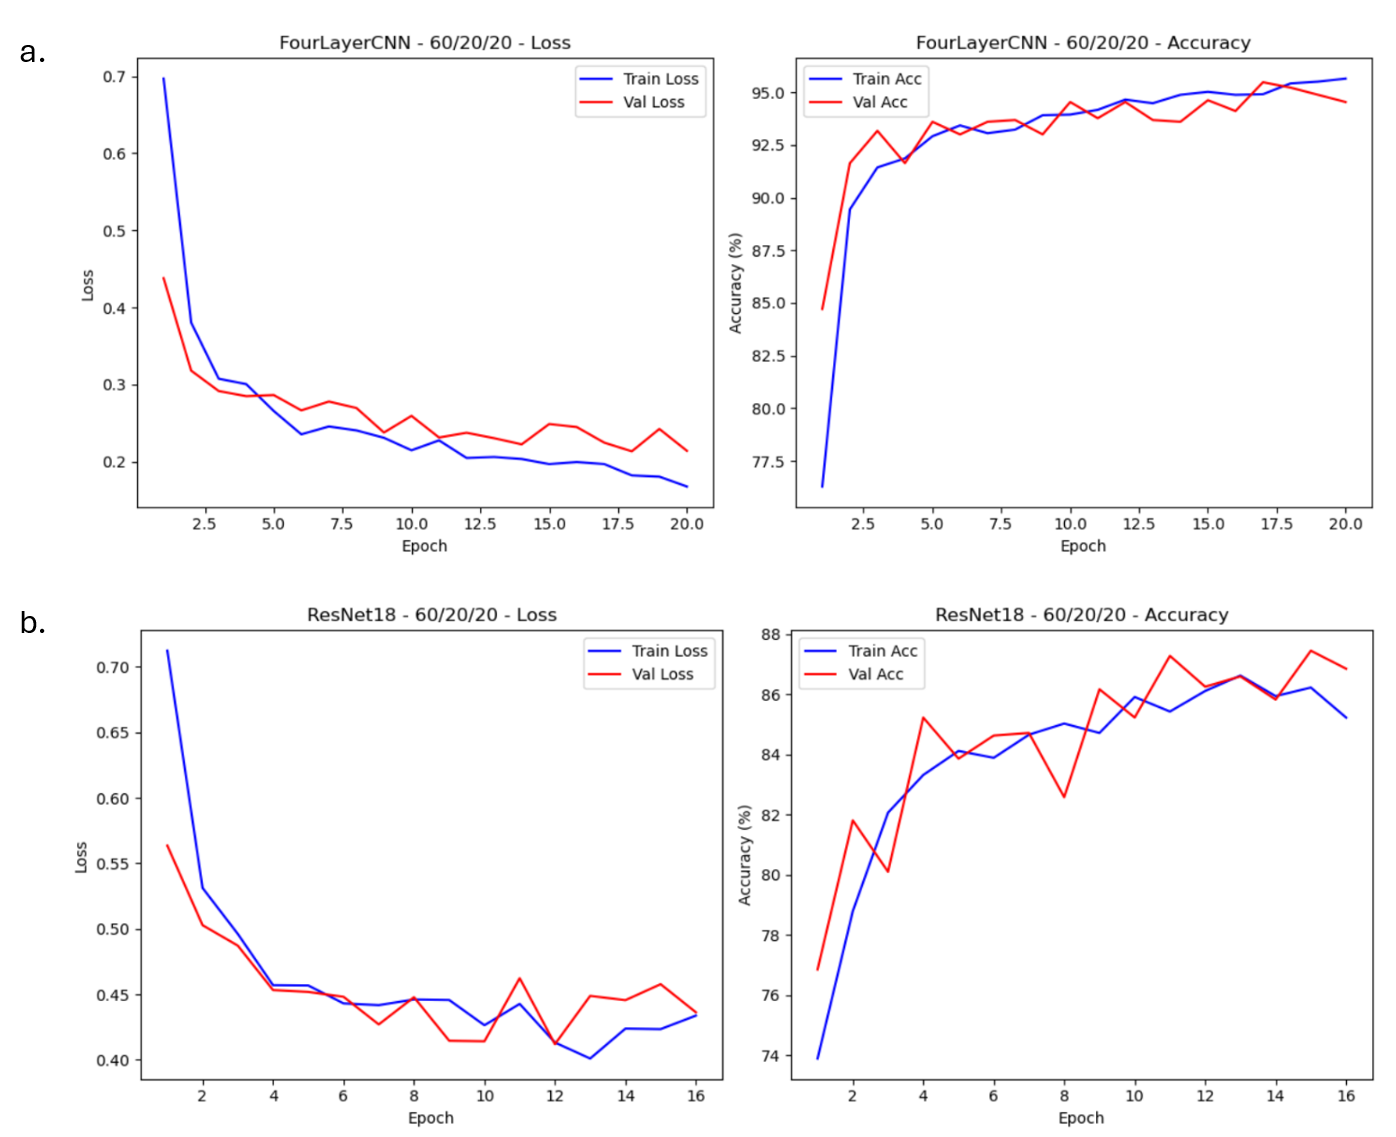
\includegraphics[width=0.90\textwidth]{./Figures/1.png} % Bildpfad ggf. anpassen
    \caption[Training and validation curves of CNN and ResNet18]{
    Training and validation loss and accuracy curves for FourLayerCNN (a.) and ResNet18 (b.) on the 60/20/20 split.
    }
    \label{fig:training_curves}
\end{figure}

\subsection{Classification Metrics}

Table~\ref{tab:metrics_summary} shows the final evaluation metrics for both models on the internal and external datasets. The FourLayerCNN outperformed ResNet18 in every metric. On the internal test set, it reached 94.45\% accuracy and a high recall of 98.57\%, resulting in an F1-score of 96.24\%. On the external dataset, it still achieved 91.11\% accuracy and an F1-score of 91.49\%, indicating strong generalization.

\vspace{0.2cm}In contrast, ResNet18 achieved 87.97\% accuracy and 92.03\% F1-score on the internal test set, but dropped to 79.44\% accuracy and 77.02\% F1-score on the external set. This drop highlights weaker robustness compared to FourLayerCNN.

\begin{table}[H]
    \centering
    \caption[Evaluation Results Summary]{Evaluation metrics for FourLayerCNN and ResNet18 across internal and external splits.}
    \label{tab:metrics_summary}
    \begin{tabular}{|l|c|c|c|c|l|}
        \hline
        \textbf{Model} & \textbf{Accuracy} & \textbf{Precision} & \textbf{Recall} & \textbf{F1-score} & \textbf{Split} \\
        \hline
        FourLayerCNN & 94.45\% & 94.00\% & 98.58\% & 96.24\% & 60/20/20 \\
        FourLayerCNN & 91.11\% & 87.76\% & 95.56\% & 91.49\% & external \\
        ResNet18     & 87.97\% & 87.82\% & 96.68\% & 92.04\% & 60/20/20 \\
        ResNet18     & 79.44\% & 87.32\% & 68.89\% & 77.02\% & external \\
        \hline
    \end{tabular}
\end{table}

\subsection{ROC Curves and AUC Scores}

The ROC curves in Figure~\ref{fig:roc} illustrate model performance in terms of classification thresholds. FourLayerCNN achieved excellent class separation with an Area Under Curve (AUC) of 0.98 for both internal and external data. ResNet18 performed slightly worse, achieving an AUC of 0.95 internally and 0.88 externally. This confirms the superior discriminative ability of the custom CNN across both seen and unseen datasets.

\begin{figure}[H]
    \centering
    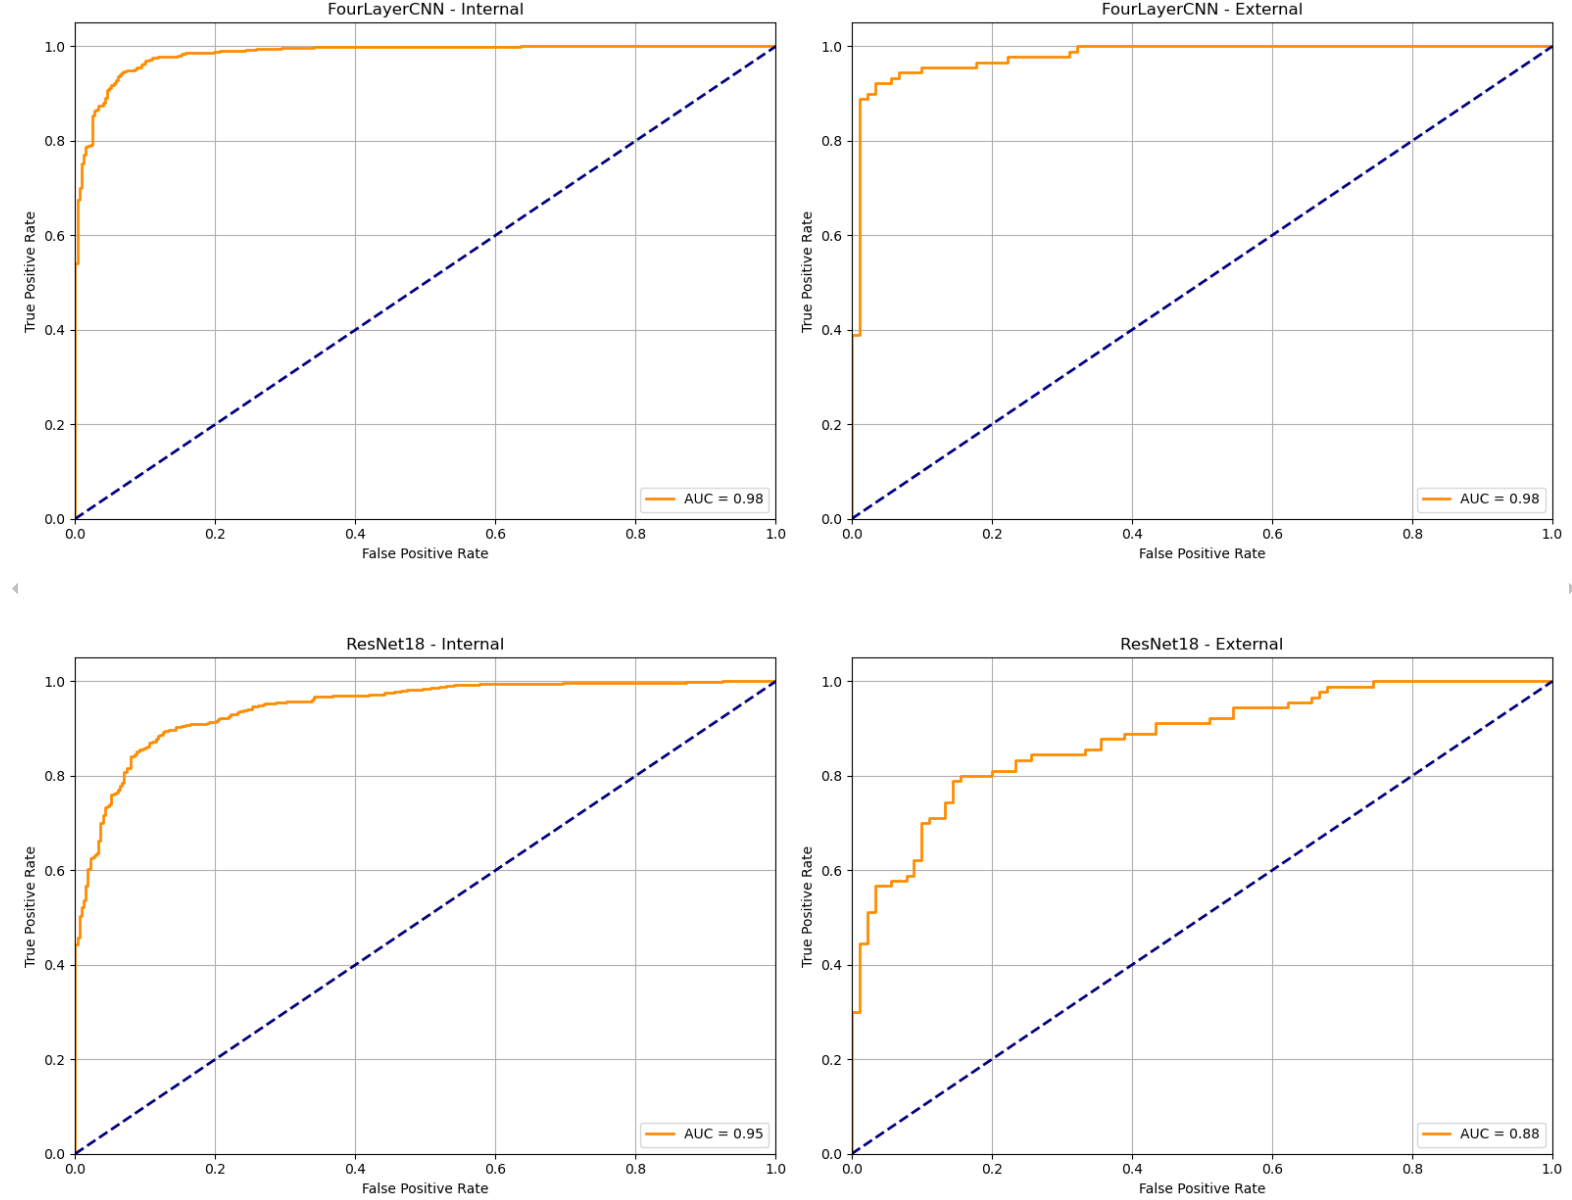
\includegraphics[width=0.90\textwidth]{./Figures/2.png} % Pfad ggf. anpassen
    \caption[ROC curves for FourLayerCNN and ResNet18]{
        ROC curves showing classification performance for both models. \textbf{Top:} FourLayerCNN, AUC = 0.98 (left: internal, right: external). \textbf{Bottom:} ResNet18, AUC = 0.95 (internal) and 0.88 (external).
    }
    \label{fig:roc}
\end{figure}

\subsection{Confusion Matrices}

Figure~\ref{fig:confusion} shows the confusion matrices for both models on the internal 60/20/20 split. FourLayerCNN made fewer false positive and false negative predictions, achieving more balanced classification results. ResNet18 showed a higher tendency to misclassify normal cases as pneumonia, resulting in lower precision and accuracy.

\begin{figure}[H]
    \centering
    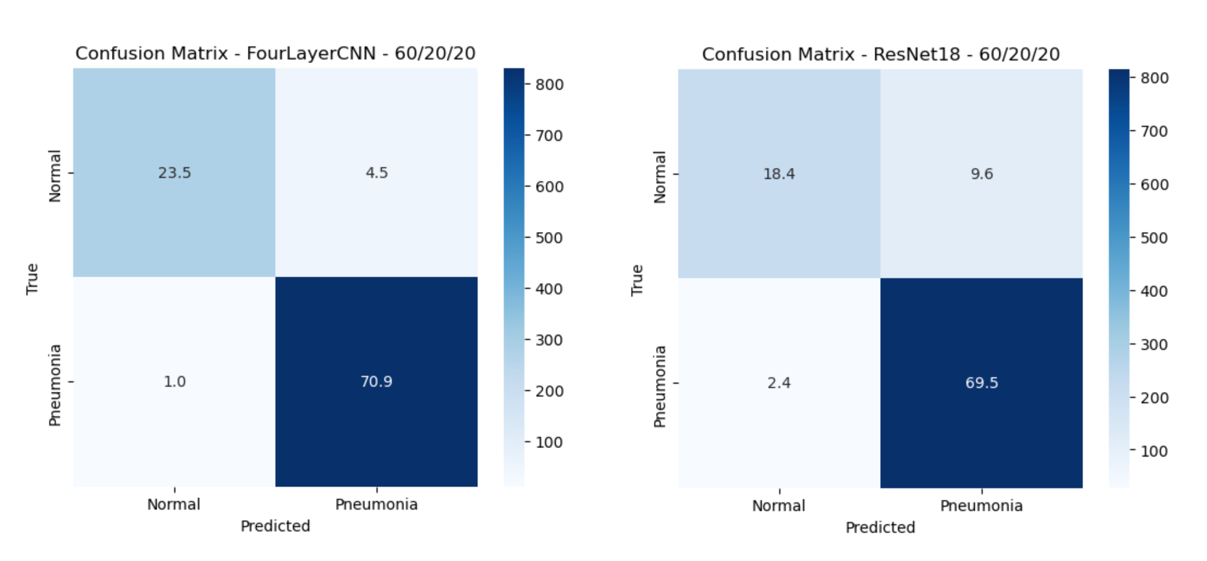
\includegraphics[width=0.85\textwidth]{./Figures/3.png} % Pfad ggf. anpassen
    \caption[Confusion matrices of FourLayerCNN and ResNet18 models]{
        Confusion matrices for internal evaluation (60/20/20 split). \textbf{Left:} FourLayerCNN. \textbf{Right:} ResNet18. FourLayerCNN demonstrates fewer misclassifications and more balanced predictions.
    }
    \label{fig:confusion}
\end{figure}

\subsection{Overall Comparison}

Figure~\ref{fig:overall_comparison} summarizes model performance in terms of accuracy and F1-score. FourLayerCNN consistently outperformed ResNet18 across all evaluation splits, particularly in external testing, which is crucial for real-world deployment. While both models performed well on the internal set, FourLayerCNN proved to be more robust and reliable on unseen data.

\begin{figure}[H]
    \centering
    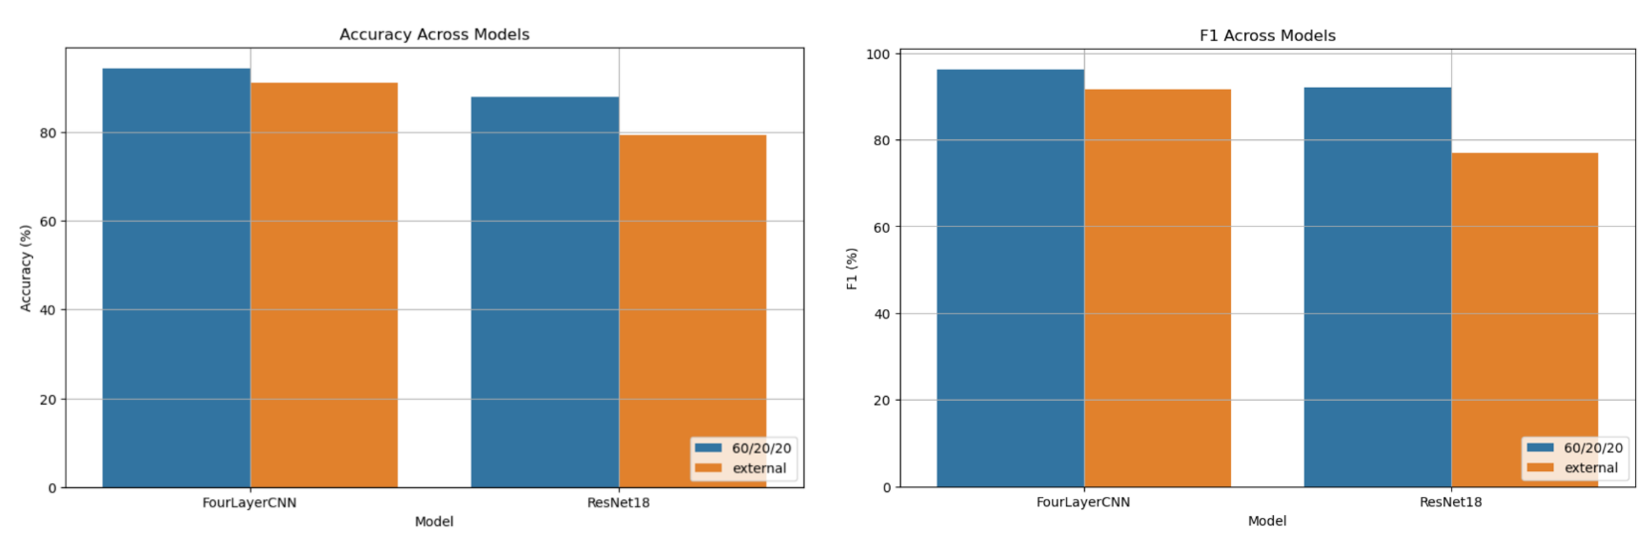
\includegraphics[width=0.95\textwidth]{./Figures/4.png} % Pfad ggf. anpassen
    \caption[Comparison of Accuracy and F1-score across splits]{
        Overall performance comparison. \textbf{Left:} Accuracy of both models on internal and external datasets. \textbf{Right:} F1-scores show FourLayerCNN performs better, especially in generalization.
    }
    \label{fig:overall_comparison}
\end{figure}

\section{Discussion}

This project demonstrated that the custom-built FourLayerCNN consistently outperformed the pre-trained ResNet18, especially when tested on external validation data. This is a key advantage for real-world clinical applications, where models must generalize well to unseen data.

\vspace{0.2cm}The simpler architecture of the FourLayerCNN likely contributed to its robustness. With fewer parameters and the use of Dropout (but no Batch Normalization), the model was less prone to overfitting. Real-time data augmentation and a weighted loss function (\texttt{pos\_weight} in \texttt{BCEWithLogitsLoss}) also helped the model learn effectively despite the class imbalance.

\vspace{0.2cm}
In contrast, ResNet18 showed more unstable training behavior and lower performance on external data. Although the input layer was modified to accept grayscale images, the model was originally trained on natural RGB images (ImageNet). This domain mismatch likely limited its ability to extract useful features from X-rays. As a result, ResNet18 tended to overpredict pneumonia and showed a higher false-positive rate.

\vspace{0.2cm}
These findings are also reflected in the confusion matrices and evaluation metrics. The FourLayerCNN performed more consistently and made fewer classification mistakes, especially for the Normal class. It achieved higher accuracy and F1-scores across all datasets and splits.

\vspace{0.2cm}
Table~\ref{tab:metrics_summary} in the Results section summarizes the evaluation metrics. It shows that FourLayerCNN achieved better scores across almost all key indicators, particularly on the external dataset, where generalization matters most.

\vspace{0.2cm}It should also be noted that the codebase was improved after the project presentation. These changes enhanced structure, visualizations, and evaluation, which improved model interpretation.

\vspace{0.2cm}Another open point was the unclear origin of the X-ray data. While metadata like patient age was not available, it is likely that most images in both datasets show pediatric cases, which is consistent with the disease's high incidence in young children.

\vspace{0.2cm}Despite strong results, some cases remained difficult to classify, likely due to visual similarity or labeling noise. The class imbalance, although addressed, may also still impact predictions.

\vspace{0.2cm}Despite these promising results, there are still challenges. Some X-ray images are difficult to classify due to visual similarities, unclear boundaries, or possible labeling errors. In addition, the dataset remains unbalanced, with more pneumonia cases than normal ones. Although this was addressed during training, the imbalance may still affect the models’ behavior in borderline cases.

\vspace{0.2cm}To improve future models, several strategies could be useful:
\begin{itemize}
    \item Collecting more and better-balanced data to support more accurate learning.
    \item Fine-tuning transfer learning models such as ResNet18 instead of freezing all layers, or testing newer architectures like EfficientNet or Vision Transformers (ViTs).
    \item Using model explainability techniques such as Grad-CAM to visualize which areas of the image were important for the decision.
    \item Testing the models on additional external datasets from other hospitals or imaging devices to validate their robustness.
\end{itemize}

\section{Conclusion}
This project demonstrated that deep learning methods can be effectively applied to detect pneumonia in pediatric chest X-rays, even when working with relatively simple architectures. The custom-built FourLayerCNN consistently outperformed a modified ResNet18, especially in generalization to external datasets. Key success factors included targeted preprocessing, data augmentation, and handling class imbalance through weighted loss functions

\vspace{0.2cm}Even though the results were good, there are still some problems. For example, the data set had little additional information about the patients, and some images may have been labeled incorrectly. In addition, the number of normal and pneumonia images was not balanced.

\vspace{0.2cm}In the future, we could try newer models, get better and more balanced data, and use tools that show which parts of the image the model uses to make decisions.

\vspace{0.2cm}Finally, our results underline the need of domain-specific model construction and thorough evaluation throughout several data sources as well as the possibilities of tailored convolutional networks for medical imaging tasks.


\newpage
\printbibliography

\renewcommand{\familydefault}{\sfdefault}  
\thispagestyle{empty}
\listoffigures
\renewcommand{\familydefault}{\sfdefault}  
\thispagestyle{empty}
\listoftables
\renewcommand{\familydefault}{\sfdefault}  
\thispagestyle{empty}
\end{document}